\documentclass{scrreport}
\usepackage[utf8]{inputenc}
\usepackage{float} 
\usepackage{graphicx}
\usepackage{hyperref}

% Add any additional packages you may need here

\renewcommand*{\thesection}{\Roman{section}}
\renewcommand*{\thesubsection}{\arabic{subsection}}
\renewcommand*{\thesubsubsection}{\roman{subsubsection}}

\title{EcoMandala: Hexagonal NFTs for Geospatial Data Integrity on Cardano}
\subtitle{Milestone Report}

\author{Team Sentinel}
\date{\today}

\graphicspath{Images/}

\begin{document}

\maketitle

\tableofcontents

\chapter*{Executive Summary}
\label{chap:executive summary}

The EcoMandala project on the Cardano blockchain utilizes hexagonal NFTs to enhance geospatial data integrity across multiple sectors. These NFTs, acting as digital passports, encapsulate detailed environmental data, promoting sustainable practices and robust data management. Key applications include:
\begin{itemize}
    \item Satellite Oracles: Enhancing the accuracy of environmental monitoring and disaster management, with real-world applications in deforestation tracking.
    \item Environmental Compliance: Enabling businesses and regulatory bodies to adhere to environmental standards with verifiable, transparent data.
    \item Sustainable Agriculture: Facilitating precision agriculture through real-time data, optimizing resource management, and improving crop yields.
    \item Disaster Response: Supporting efficient emergency operations with timely geospatial data, enhancing the effectiveness of disaster relief and recovery.
    \item Urban Planning: Guiding sustainable urban and infrastructure development through detailed environmental assessments.
    \item Carbon Credits: Assisting in the accurate monitoring and verification of carbon sequestration projects, fostering trust in global carbon markets.
    
\end{itemize}


This project underscores the potential of integrating blockchain technology with environmental conservation efforts, offering significant benefits to diverse stakeholders including governmental agencies, NGOs, and businesses in forestry and agriculture. The comprehensive application of these NFTs paves the way for improved environmental governance and more informed decision-making processes across industries.


\chapter*{Introduction}
\label{chap:introduction}
EcoMandala's hexagonal NFTs on the Cardano blockchain aim to secure geospatial data integrity, focusing on environmental monitoring and conservation. Utilizing NMKR, these NFTs serve as "digital passports" for specific land units, encapsulating environmental data and history to support sustainability efforts. The data structure is organized into hexagonal units using the Uber H3 grid, providing detailed environmental insights for each location. The project is designed to promote data verification, environmental DApps development, and broader blockchain adoption in sectors requiring reliable data management.

This document will present some of the potential target Use Cases for EcoMandala’s Hexagonal NFTs on Cardano.
\chapter{Potential Use Cases for EcoMandala's Hexagonal NFTs on Cardano}
\label{chap:use_cases}

\section{Enhanced Geospatial Data Integrity for Satellite Oracles}
\label{chap:geospatial_data_integrity}

This application ensures the accuracy and security of data used for environmental monitoring, disaster management, and resource allocation.

The application of Enhanced Geospatial Data Integrity through satellite oracles significantly boosts the reliability of environmental data. This is crucial for sectors like environmental monitoring, disaster management, and resource allocation. By integrating satellite oracles with blockchain technology, such as through EcoMandala’s hexagonal NFTs, each piece of data is verified and secured. This ensures that the data used in monitoring environmental changes, responding to natural disasters, or managing natural resources is accurate, tamper-proof, and readily available for decision-makers. This integrity is vital for planning effective interventions and policies, providing a foundation for trustworthy data-driven decisions.

A real-world example of enhanced geospatial data integrity using satellite oracles involves tracking deforestation in critical areas like the Amazon Rainforest. By using blockchain-secured satellite data, organizations can detect unauthorized logging activities in real-time. This data, confirmed through immutable NFTs, enables swift action from authorities and helps in the planning of reforestation efforts. Such precise and trusted data is essential for maintaining ecological balance and enforcing environmental policies effectively.
In the Amazon Rainforest, satellite oracles integrated with EcoMandala’s hexagonal NFTs offer a robust solution for tracking deforestation activities. Each NFT represents a specific hexagonal segment of the forest, with satellite imagery providing frequent updates on this segment’s condition. When unauthorized logging is detected within a segment, the corresponding NFT records and verifies this activity securely on the blockchain. This process not only allows for immediate detection but also facilitates rapid response from local authorities and conservation groups, who can access this data to enforce laws and plan recovery operations efficiently. This real-time, transparent monitoring system enhances accountability and aids in sustainable forest management, crucial for the preservation of biodiversity and mitigation of climate change impacts.

In the Amazon Rainforest example using EcoMandala's hexagonal NFTs, various ecosystem players utilize the enhanced geospatial data integrity in different ways:
\begin{enumerate}
    \item Environmental NGOs and Researchers: Analyze the data to monitor biodiversity and ecosystem health, creating reports that influence policy and awareness.
    \item Government Agencies: Use the data for enforcement and regulatory purposes, detecting illegal activities and ensuring compliance with environmental laws.
    \item Local Communities and Indigenous Groups: Leverage this data to protect their lands and maintain sustainable practices.
    \item Businesses in Forestry and Agriculture: Might use the data to plan sustainable land use and to prove sustainable practices for certification and market advantage.
    \item Technology Developers and Data Analysts: Create and refine algorithms that better interpret satellite data for more accurate and actionable insights, feeding into broader conservation strategies.
\end{enumerate}

Each player's use of the data underscores a collaborative approach to managing and preserving the Amazon Rainforest, showcasing the potential of technology in environmental conservation efforts.

This can attract investment from governmental and environmental bodies seeking robust data management solutions. Companies specializing in satellite technology and data analytics can also leverage these oracles to improve service offerings.

\section{Improved Environmental Compliance and Reporting}

The satellite oracles project highlights the potential for using hexagonal NFTs to enhance transparency and reliability in environmental compliance and reporting. Businesses and regulatory bodies can utilize this verified data to adhere to environmental standards and policies.

In the context of the Amazon Rainforest, the use of EcoMandala’s hexagonal NFTs for enhanced environmental compliance and reporting allows businesses and regulatory bodies to access accurate, verified data on deforestation and land use changes. This data can be critical for ensuring compliance with environmental policies, such as those governing sustainable logging practices and land development restrictions. For example, a timber company may use this reliable data to demonstrate adherence to legal cutting practices, while government agencies can monitor and enforce these regulations more effectively, ensuring environmental standards are met.

For a specific example, consider a scenario involving a multinational corporation operating in the timber industry. This corporation could use data verified by satellite oracles to ensure that their operations comply with sustainable harvesting laws. The NFTs would provide immutable evidence of the corporation's adherence to environmental standards, which they can present during audits and public disclosures. Regulatory bodies could then use this data to monitor compliance across the industry, facilitating faster and more targeted enforcement actions against non-compliance. This setup enhances transparency, builds trust with stakeholders, and ensures that environmental policies are effectively upheld.

In the context of improved environmental compliance and reporting:
\begin{enumerate}
    \item Regulatory Agencies: They will utilize the data from hexagonal NFTs to monitor adherence to environmental laws across industries like forestry and mining, enhancing enforcement and reducing illegal activities.
    \item Corporations in High-Impact Sectors: Businesses, especially in sectors with significant environmental footprints such as manufacturing and agriculture, will use these NFTs to track and report on their environmental performance, ensuring compliance with regulations.
    \item Environmental Auditors and Consultants: These professionals will rely on the accurate and immutable data provided by the NFTs to audit corporate compliance with environmental standards, offering services to help businesses maintain or achieve compliance.
\end{enumerate}
These players will use the secure, transparent data from the EcoMandala project to improve the quality of environmental reporting and ensure that compliance is both verifiable and based on reliable data.

There's potential for collaboration with corporate entities needing to demonstrate compliance with environmental regulations, potentially opening up new markets for software and consulting services.

\section{Support for Sustainable Agriculture}

Integrating EcoMandala’s NFTs with real-time satellite data can transform agricultural practices by enabling precise field boundary detection, crop classification, and yield prediction. This supports sustainable agriculture initiatives by providing farmers with actionable insights to optimize crop management and reduce environmental impact.

For instance, farmers can access geospatial data stored on these NFTs to monitor and manage land use effectively. This data can include detailed information about soil health, moisture levels, and crop growth across different farm segments. Precision agriculture techniques can then be applied, allowing for optimal irrigation, fertilization, and pest management based on the specific needs of each hexagonal unit. This targeted approach helps in maximizing yields, reducing waste, and minimizing environmental impact, promoting a more sustainable agricultural practice overall.

Incorporating the EcoMandala project into sustainable agriculture offers significant benefits for finance and insurance sectors. Financial institutions can use verified geospatial data to assess the viability and sustainability of agricultural investments, leading to more informed lending decisions. Meanwhile, insurance companies can leverage this precise data to tailor insurance products, setting premiums based on the actual conditions and risks of specific farm areas. This approach minimizes financial risks and supports farmers committed to sustainable practices, creating a more resilient agricultural sector.

For microfinance, financial institutions can use detailed geospatial data to assess the risk and potential of small-scale farming operations, enabling them to offer more tailored financial products. In microinsurance, insurers can utilize the same data to accurately price premiums based on specific environmental risks, such as drought or flooding, at a granular level. This targeted approach can make financial and insurance services more accessible and affordable for smallholder farmers, fostering financial inclusion and risk management in rural areas.

In supporting sustainable agriculture, various ecosystem players can utilize hexagonal NFTs as follows:
\begin{enumerate}
    \item Farmers and Agricultural Producers: These primary users will leverage real-time, precise data to enhance crop yields, manage resources more efficiently, and implement sustainable practices tailored to specific plot needs.
    \item Agricultural Technologists and Agri-tech Companies: They can develop new tools and applications based on the accurate, reliable data from NFTs, enhancing precision farming solutions.
    \item Government and Policy Makers: Utilizing the data for crafting policies that promote sustainable agricultural practices and for monitoring compliance with agricultural standards.
\end{enumerate}
These players benefit from precise, reliable data to drive efficiency, sustainability, and compliance in agriculture.

This use case could see interest from agri-tech firms, sustainability-focused NGOs, and governments aiming to boost agricultural productivity while minimizing environmental impact. It also opens avenues for precision farming technology providers.

\section{Disaster Response and Management}
The EcoMandala project can significantly enhance disaster response and management by providing real-time, accurate geospatial data through its hexagonal NFTs. For instance, in flood-prone regions, the system can deliver up-to-the-minute information on water levels and land saturation across different hexagons. This data can be crucial for emergency services to prioritize response efforts, deploy resources more efficiently, and execute timely evacuations. Additionally, post-disaster recovery can be better managed by assessing the damage through updated satellite data, aiding in quicker and more effective rebuilding efforts. This application ensures a rapid and targeted response, potentially saving lives and reducing economic impacts.

Consider a scenario involving a hurricane approaching a coastal region. The hexagonal NFTs can provide up-to-date information on wind speeds, storm surge levels, and flooding risks specific to each hexagonal grid area. This data allows emergency response teams to prioritize areas that are most at risk and plan evacuation routes effectively. Furthermore, after the storm, this data helps assess the extent of damage for rapid deployment of aid and reconstruction resources, ensuring resources are directed where they are most needed. This real-time data is invaluable for minimizing the impact of natural disasters and accelerating recovery efforts.

Various ecosystem players would use hexagonal NFTs in the following ways:
\begin{enumerate}
    \item Emergency Response Teams: Utilizing real-time data from the NFTs for effective disaster response planning and operations, ensuring quick and targeted assistance.
    \item Government Agencies: Leveraging this data for resource allocation, disaster preparedness, and to efficiently coordinate with other agencies and non-governmental organizations.
    \item Non-Governmental Organizations (NGOs): Using accurate, updated data to prioritize aid and reconstruction efforts, maximizing the impact of their resources in affected areas.
\end{enumerate}

These players depend on immediate, reliable data to manage crises and optimize disaster response and recovery efforts.

Disaster management agencies, humanitarian organizations, and insurance companies could benefit from more accurate disaster response planning and assessment capabilities.

\section{Carbon Credits and Environmental Impact Monitoring}

The integration of EcoMandala’s NFTs with satellite oracles could significantly enhance the monitoring and verification processes for carbon credit systems. By providing reliable data on environmental impacts, these NFTs support global efforts in climate change mitigation.

The EcoMandala project can be instrumental in the field of carbon credits and environmental impact monitoring. By using the detailed geospatial data from hexagonal NFTs, organizations can monitor and verify carbon sequestration projects more accurately. For instance, a company might initiate a reforestation project and use the NFTs to track the growth and health of newly planted areas over time. This verified data can be used to issue carbon credits, with each NFT serving as a transparent and immutable record of the carbon captured. This system not only enhances trust in carbon trading markets but also ensures that environmental impacts are monitored and managed effectively.

For carbon credits and environmental impact monitoring:
\begin{enumerate}
    \item Environmental Regulators: They would use the data from hexagonal NFTs to verify the accuracy of reported carbon sequestration efforts, ensuring compliance with international climate agreements.
    \item Corporations: Companies looking to offset their carbon footprint would use this data to invest in verified carbon credit projects, showcasing their commitment to sustainability.
    \item Conservation Organizations: These groups can utilize the data to monitor and report on the effectiveness of conservation efforts, helping to secure funding and support from donors.
\end{enumerate}

This ties directly into the global carbon credit market, appealing to companies under pressure to meet environmental targets, and those facilitating carbon trading.


\chapter{The PoC Project}
\label{chap:project}

\section{Proposed Architecture}

The following EcoMandala system architecture describes the flow of data from the tasking, collection and processing to its storage and interaction with the blockchain, as well as its use in various applications.

\begin{enumerate}
    \item Data Collection Layer

    Components:
    \begin{description}
        \item[Satellite Sensors:] Captures multispectral imaging data.
        \item[Climate Data Sensors:] Collects temperature, precipitation, and cloud cover data.
        \item[Field Sensors:] Collects soil health, moisture levels, and other on-the-ground environmental data.
    \end{description}
    Description: This layer represents the sources of environmental data, including satellite imaging, climate sensors, and field data.

    \item Data Ingestion and Processing Layer

    Components:
    \begin{description}
        \item[Data Ingestion Pipeline:] Handles the collection of raw data from various sensors.
        \item[Data Preprocessing Unit:] Performs radiometric calibration, cloud removal, and other preprocessing tasks to clean and prepare the data.
        \item[Hexagonal Grid Mapping (Uber H3):] Maps environmental data onto a hexagonal grid based on the Uber H3 system.
    \end{description}
    Description: This layer is responsible for ingesting raw data and preprocessing it into a standardized format, mapped onto hexagonal units.

    \item Blockchain Interaction Layer
    
    Components:
    \begin{description}
        \item[NFT Generation Module (NMKR):] Creates NFTs representing each hexagonal unit.
Smart Contracts: Governs the minting, updating, and transaction of NFTs.
        \item[Blockchain Network (Cardano):] Stores the NFTs and associated environmental data securely and immutably.
    \end{description}
    Description: This layer depicts how processed environmental data is encapsulated into NFTs, which are then minted and managed on the Cardano blockchain.

    \item{Data Access and Interaction Layer}

    Components:
    \begin{description}
        \item[API Gateway:] Provides access to NFT data and environmental insights through standardized APIs.
        \item[User Interface (UI):] A front-end interface for end-users to interact with the data, view NFTs, and analyze environmental conditions.
    \end{description}
    Description: This layer represents how end-users and applications access the environmental data stored on the blockchain through APIs and user interfaces.

    \item Application Layer

    Components:
    \begin{description}
        \item[Environmental Monitoring Dashboards:] Tools for visualizing environmental data and trends.
        \item[Compliance Reporting Tools:] Applications that generate reports for environmental compliance.
        \item[Disaster Management Systems:] Interfaces and tools for real-time disaster monitoring and response.
        \item[Sustainable Agriculture Platforms:] Tools that leverage data for precision farming and resource management.
        \item[Carbon Credit Verification Systems:] Applications that track and verify carbon sequestration projects.
    \end{description} 
    Description: This layer illustrates the various applications that utilize the data from the EcoMandala service for different use cases.

\end{enumerate}

Flow of Information:

\begin{description}

    \item{Data Collection:} Environmental data is gathered from satellite, climate, and field sensors.

    \item{Data Ingestion and Processing:} The raw data is cleaned, preprocessed, and mapped onto a hexagonal grid.

    \item{Blockchain Interaction:} Processed data is encapsulated into NFTs, which are then minted and stored on the Cardano blockchain.

    \item{Data Access and Interaction:} End-users access this data through APIs and user interfaces, interacting with the NFTs and underlying environmental data.

    \item{Application Use:} Various applications use this data for monitoring, compliance, disaster management, sustainable agriculture, and carbon credit verification.

\end{description}

These diagrams collectively detail the structural and operational nuances of the Security Oracle framework and its integration with the Cardano blockchain.

\begin{itemize}
    \item Figure \ref{fig:components_diagram} presents the main layers of the EcoMandala system, service architecture and data flow.
    \item Figures \ref{fig:ui-screen-1} and \ref{fig:ui-screen-2} depict the outline of the basic User Interface (UI) of the EcoMandala service.
    %\item Figure  provides a simplified overview of the data flow process, focusing on the key interactions between users, smart contracts, and the Security Oracle.
\end{itemize}

% Placeholder for Components Diagram
\begin{figure}[H]
\centering
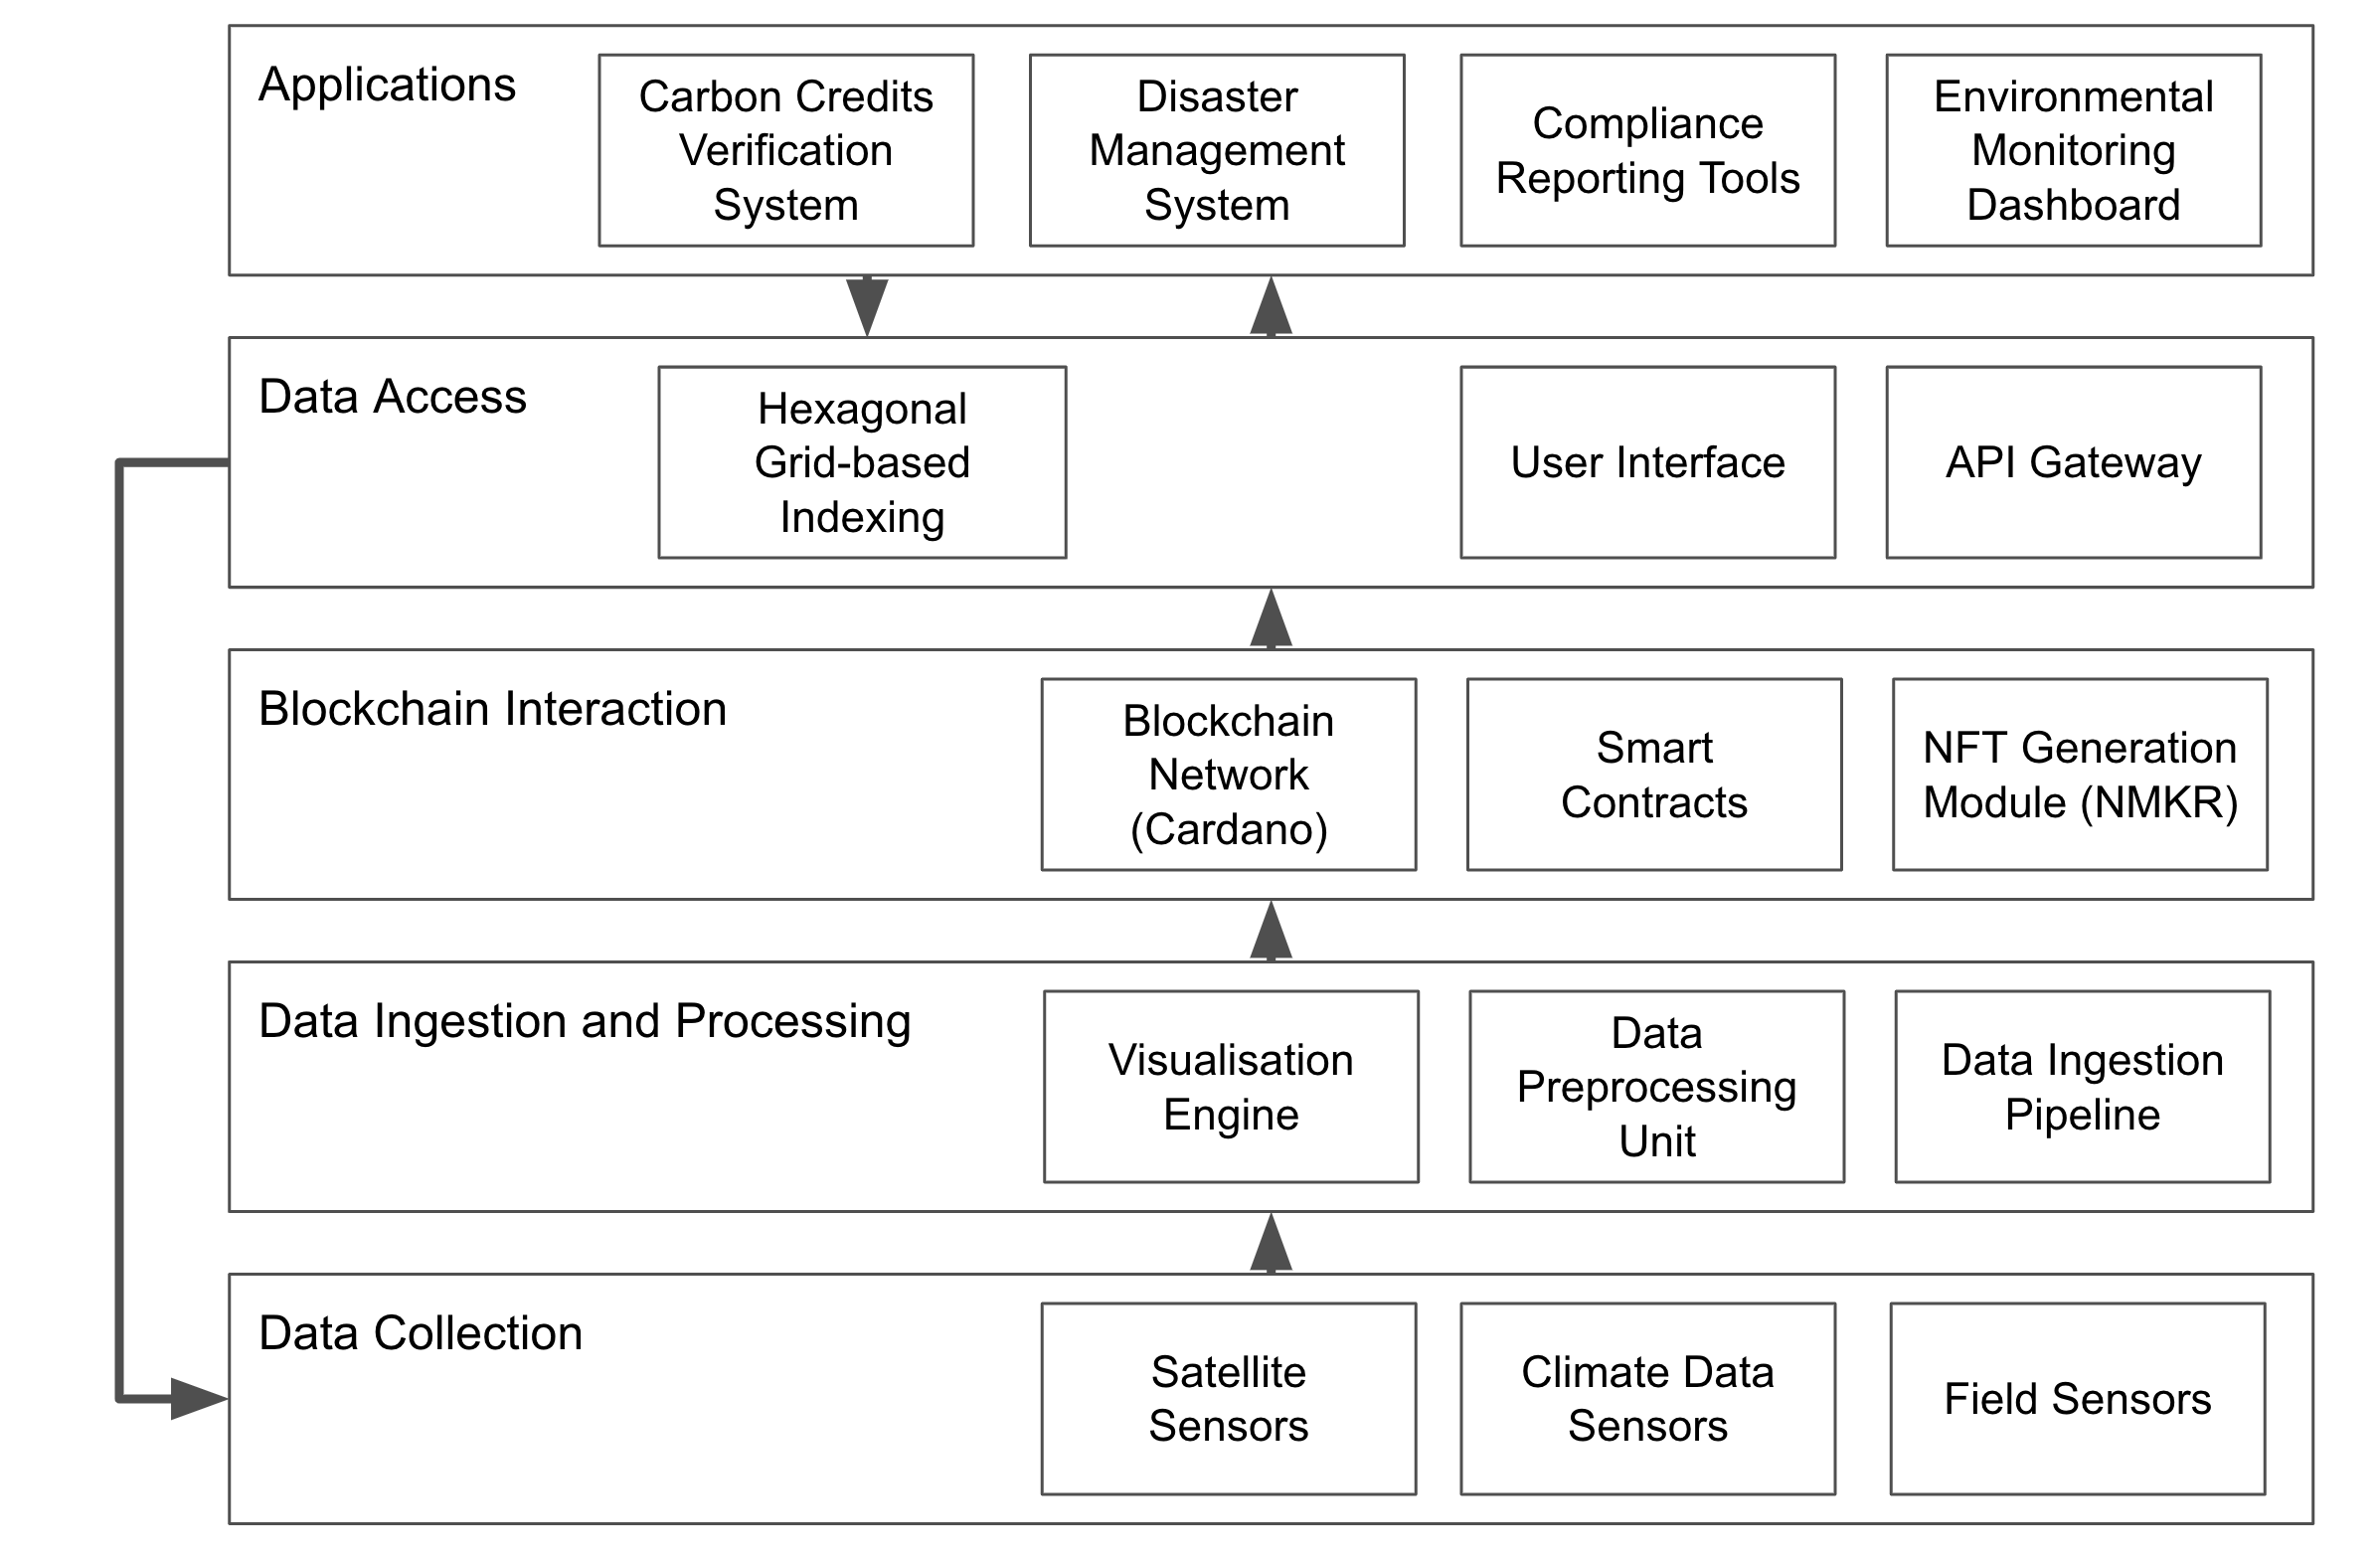
\includegraphics[width=\textwidth]{Images/ecomandala-20240912-1.png}
\caption{EcoMandala system architecture and data flow.}
\label{fig:components_diagram}
\end{figure}

\begin{figure}[H]
    \centering
    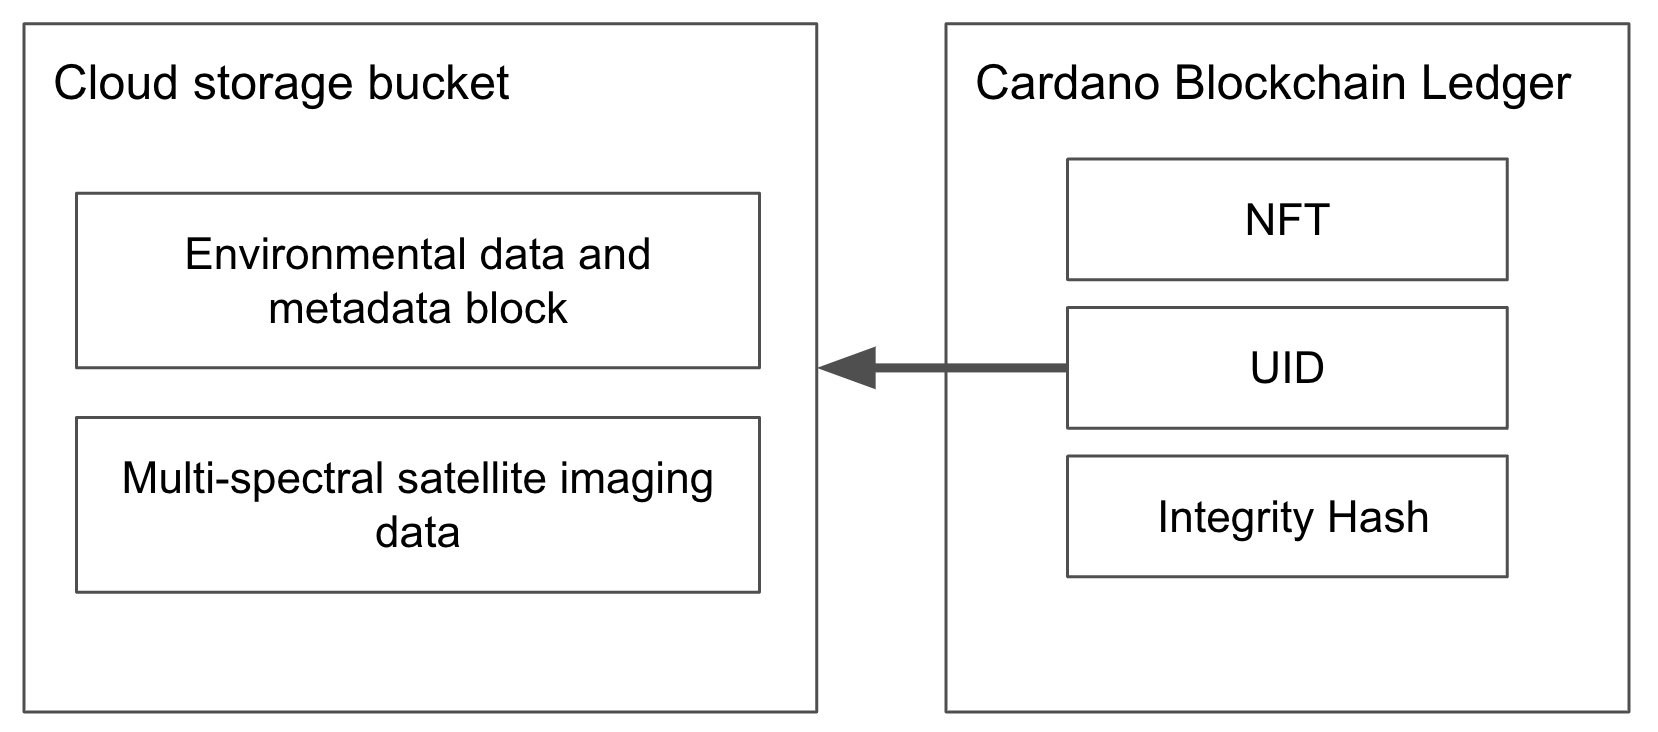
\includegraphics[width=0.8\textwidth]{Images/ecomandala-data-20240913-1.png}
    \caption{On/off chain data structure.}
    \label{fig:data-structure}
\end{figure}

% Placeholder for Dataflow Diagram with Simplified Model
\begin{figure}[H]
\centering
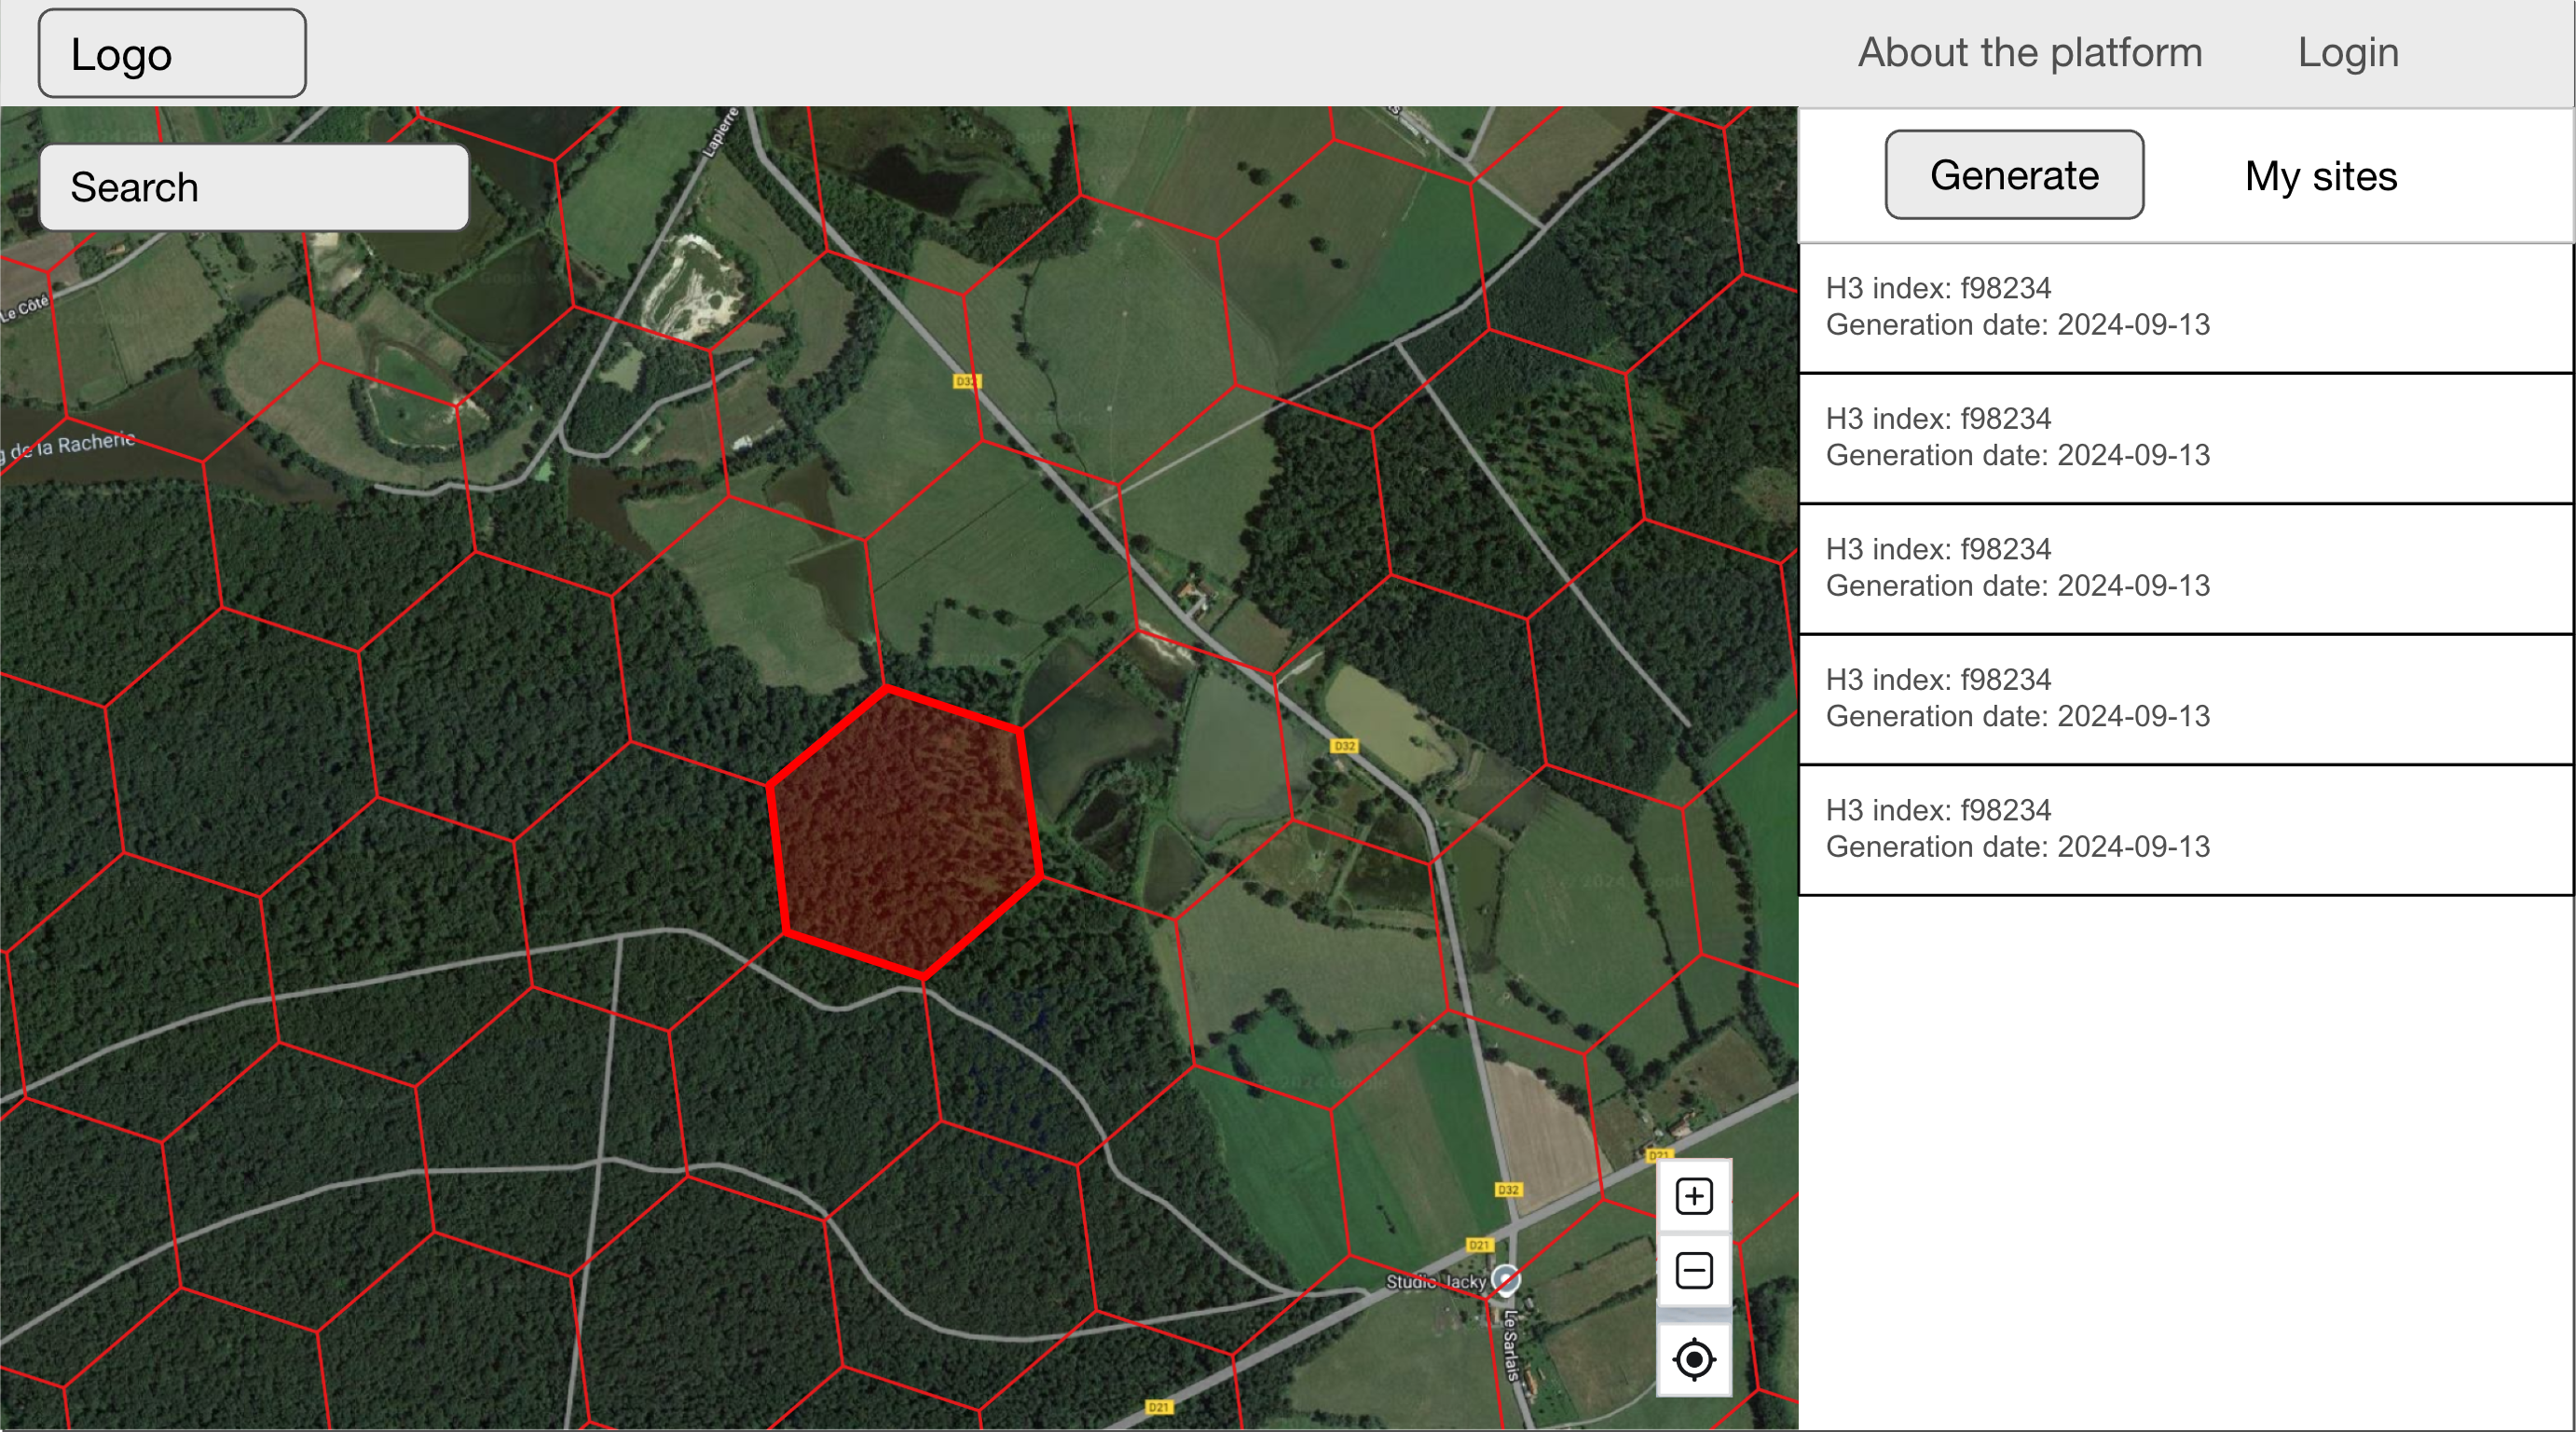
\includegraphics[width=\textwidth]{Images/screen1-20240913-1.png}
\caption{EcoMandala UI outline: Screen 1.}
\label{fig:ui-screen-1}
\end{figure}

% Placeholder for Dataflow Diagram with Pull Model
\begin{figure}[H]
\centering
\includegraphics[width=\textwidth]{Images/screen2-20240913-1.png}
\caption{EcoMandala UI outline: Screen 2.}
\label{fig:ui-screen-2}
\end{figure}

\newpage
\subsection{Data Structure}
The following JSON schema will be utilised to store environmental data for each of the sites
\begin{verbatim}
{
    "$schema": "http://json-schema.org/draft-07/schema#",
    "title": "EcoMandala Data Structure",
    "type": "object",
    "properties": {
        "hexID": {
        "type": "string",
        "description": "Unique identifier for the hexagonal grid cell based on Uber H3 system."
        },
        "location": {
        "type": "object",
        "description": "Geospatial coordinates of the hexagonal unit.",
        "properties": {
            "latitude": {
            "type": "number",
            "description": "Latitude of the hexagonal grid center."
            },
            "longitude": {
            "type": "number",
            "description": "Longitude of the hexagonal grid center."
            }
        },
        "required": ["latitude", "longitude"]
        },
        "timestamp": {
        "type": "string",
        "format": "date-time",
        "description": "Timestamp of the data capture."
        },
        "environmentalData": {
        "type": "object",
        "description": "Environmental data associated with the hexagonal unit.",
        "properties": {
            "satelliteImagery": {
            "type": "object",
            "description": "Details of the satellite imagery captured.",
            "properties": {
                "imageURL": {
                "type": "string",
                "format": "uri",
                "description": "URL to the satellite image."
                },
                "resolution": {
                "type": "string",
                "description": "Spatial resolution of the image (e.g., '1m/px')."
                },
                "bands": {
                "type": "array",
                "description": "List of spectral bands captured.",
                "items": {
                    "type": "string"
                }
                }
            },
            "required": ["imageURL", "resolution", "bands"]
            },
            "climateData": {
            "type": "object",
            "description": "Climate data related to the hexagonal unit.",
            "properties": {
                "temperature": {
                "type": "number",
                "description": "Temperature in Celsius."
                },
                "precipitation": {
                "type": "number",
                "description": "Precipitation in mm."
                },
                "cloudCover": {
                "type": "number",
                "description": "Percentage of cloud cover."
                }
            },
            "required": ["temperature", "precipitation", "cloudCover"]
            },
            "soilData": {
            "type": "object",
            "description": "Soil data for the hexagonal unit.",
            "properties": {
                "moistureLevel": {
                "type": "number",
                "description": "Soil moisture level as a percentage."
                },
                "pH": {
                "type": "number",
                "description": "Soil pH level."
                },
                "nutrientLevels": {
                "type": "object",
                "description": "Concentration of key soil nutrients.",
                "properties": {
                    "nitrogen": {
                    "type": "number",
                    "description": "Nitrogen content in mg/kg."
                    },
                    "phosphorus": {
                    "type": "number",
                    "description": "Phosphorus content in mg/kg."
                    },
                    "potassium": {
                    "type": "number",
                    "description": "Potassium content in mg/kg."
                    }
                },
                "required": ["nitrogen", "phosphorus", "potassium"]
                }
            },
            "required": ["moistureLevel", "pH", "nutrientLevels"]
            }
        },
        "required": ["satelliteImagery", "climateData", "soilData"]
        },
        "nftMetadata": {
        "type": "object",
        "description": "Metadata related to the NFT representing this hexagonal unit.",
        "properties": {
            "nftID": {
            "type": "string",
            "description": "Unique identifier of the NFT on the Cardano blockchain."
            },
            "mintedTimestamp": {
            "type": "string",
            "format": "date-time",
            "description": "Timestamp when the NFT was minted."
            },
            "transactionHash": {
            "type": "string",
            "description": "Hash of the blockchain transaction that minted the NFT."
            }
        },
        "required": ["nftID", "mintedTimestamp", "transactionHash"]
        },
        "dataProvenance": {
        "type": "object",
        "description": "Information about the origin and processing of the data.",
        "properties": {
            "source": {
            "type": "string",
            "description": "Source of the data (e.g., satellite name, sensor type)."
            },
            "processingDetails": {
            "type": "string",
            "description": "Details on how the data was processed (e.g., algorithms used)."
            }
        },
        "required": ["source", "processingDetails"]
        }
    },
    "required": ["hexID", "location", "timestamp", "environmentalData", "nftMetadata", "dataProvenance"]
}
\end{verbatim}

\newpage


\section{Project Plan}

The project plan for the Security Oracles Proof of Concept (PoC) is delineated through a series of structured milestones, each with specific objectives that guide the development process from inception to completion. Below is a Gantt chart that visually represents the timeline and interdependencies of these milestones.

%\begin{figure}[H]
%\centering
%\includegraphics[width=\linewidth]{Images/Security Oracles - Project Plan.jpg}
%\caption{Gantt Chart for the Security Oracles PoC Project Plan}
%\label{fig:gantt_chart}
%\end{figure}

The Gantt chart illustrates the project's progression over a 25-week period, broken down as follows:

\begin{itemize}
  \item \textbf{Milestone 1 (Weeks 1-4):} Research and Planning, including the exploration of vulnerabilities and architectural design, culminating in the Milestone Report.
  \item \textbf{Milestone 2 (Weeks 5-12):} Oracle Proxy Implementation, where smart contracts are developed and deployed to the testnet.
  \item \textbf{Milestone 3 (Weeks 13-20):} Threat Intelligence Monitoring System is developed, with technical research and business analysis taking place to inform its implementation.
  \item \textbf{Final Milestone (Weeks 21-25):} Documentation and Closeout, where all documentation is finalized and a closeout report and video are produced.
\end{itemize}

The planned milestones are crafted to ensure that each phase of the project builds upon the last, with time allocated for the necessary research, development, testing, and documentation required to deliver a comprehensive solution for enhancing smart contract security on the Cardano blockchain.

\appendix
\chapter{References}

Our reseach included discussions with the following organizations - 
\begin{itemize}
    \item \textbf{\href{https://cardanofoundation.org/}{Cardano Foundation}} multiple teams (Finance, partnership, tech support)
    \item ...
\end{itemize}

The following articles contributed to our research - 
\begin{itemize}
    \item ...
\end{itemize}

\end{document}
